In finding the local or global extrema of a function, algorithms such as line search and golden section search can be very helpful. For this problem, we used the two algorithms to find the global minimum on the range $x = [0.01,\ 10]$ of the function

\begin{equation}
	y = 3x + log(x)
	\label{funtomin}
\end{equation}

The actual global minimum is achieved at approximately $x = 0.333$, as seen in the figure below.

\begin{figure}[H]
\centering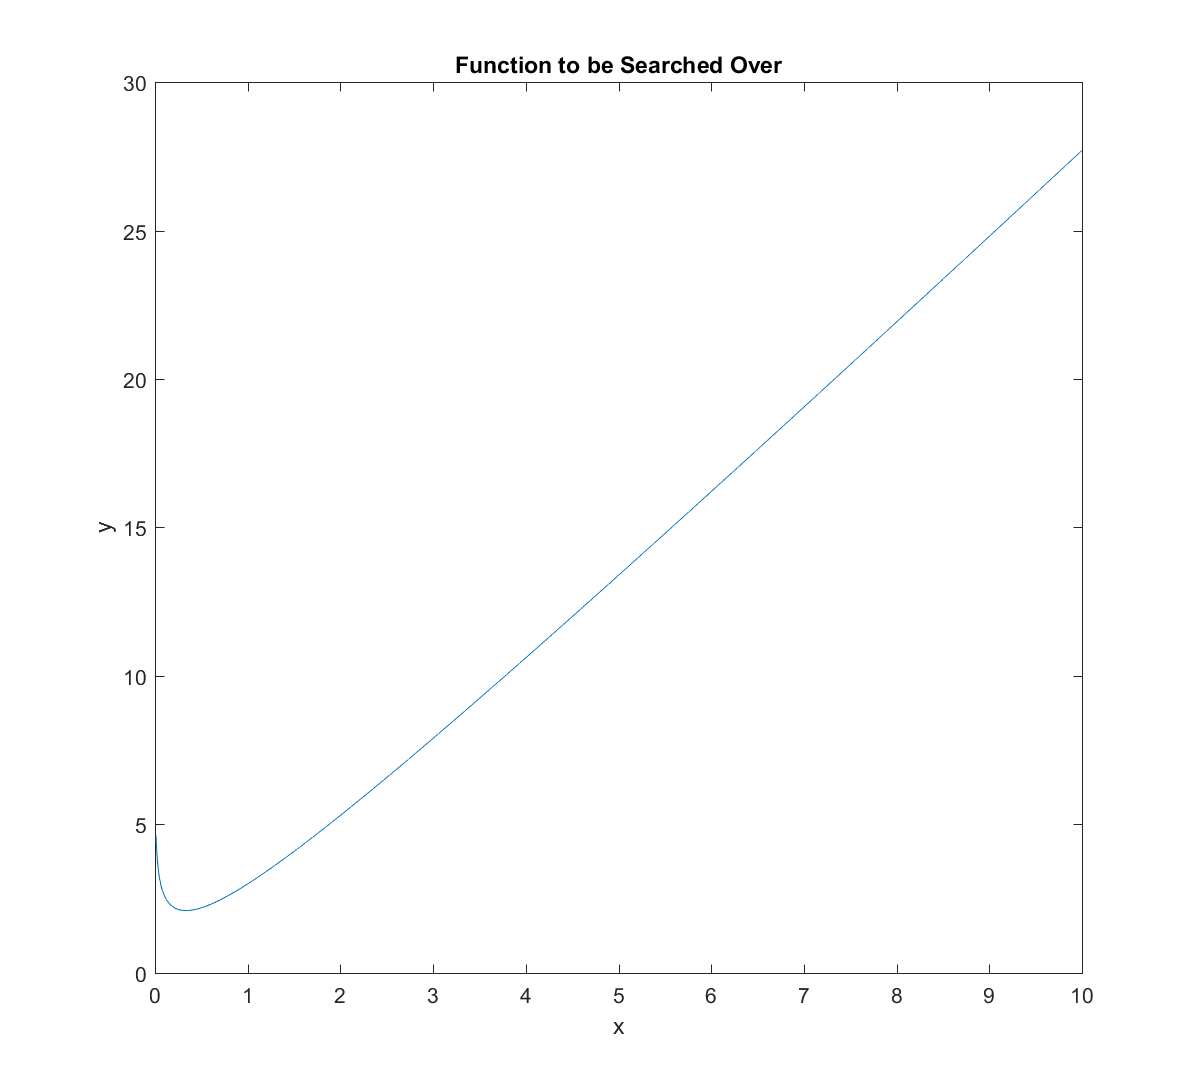
\includegraphics[width=0.6\textwidth]{function}
\caption{The function to be searched over in Problem 2.}
\end{figure}

\subsection{Line Search}

	To implement line search, we modified the example code from the course webpage. We converted line search to be a function with the signature:

	\begin{center}
	\code{function minimum = line\_search(a, b, num\_iter)}
	\end{center}
	
	\code{line\_search(.)} returns the x-value of the minimum of the function, where \code{a} and \code{b} are the minimum and maximum of the range to be searched respectively. \code{num\_iter} is the maximum number of iterations to run. This modular function allows us to easily time the line search algorithm in \code{pr2.m}.

\subsection{Golden Section Search}
	Our implementation of line search was compared against an implementation of Golden Section Search\footnote{We referenced the following Wikipedia page for our implementation: https://en.wikipedia.org/wiki/Golden-section\_search}. Golden Section search is like line search in that it proceeds iteratively over a known function; however, its advantage over line search is that it is less computationally expensive. We will discuss this advantage in the next section. We implemented golden section search with the function signature
	
	\begin{center}
	\code{function minimum = golden(a, b, tol, num\_iter)}
	\end{center}
	
	\code{golden(.)} returns the x-value of the minimum of the function, where \code{a} and \code{b} are the minimum and maximum of the range to be searched respectively. \code{tol} is one of two stop conditions for the iterations of the function. If \code{num\_iter} hasn't been reached and \code{(abs(c - d) < tol)}, then the function returns its minimum. This allows the user to specify a sort of accuracy, with a hard limit at \code{num\_iter}. In our experiment, we were essentially only using the hard limit, as \code{tol} was set to $1e-10$. This modular function allows us to easily time the line search algorithm in \code{pr2.m}.
	
	
\subsection{Performance Comparison}
	In \code{pr2.m}, we compare the speed of \code{line\_search(.)} and \code{golden(.)} over 500 executions of the same calculation. This is to obtain a stable average time for each function. We also captured the shortest execution of the 100 repetitions to get an idea for the best-case performance. Finally, we captured the absolute difference in the minimum returned by each solution. This allowed us to compare the speed and accuracy of the two functions. \code{num\_iter} was set to 10 for each algorithm. The results are illustrated in the table below.
	
	\begin{table}[H]
	\centering\makegapedcells
	\begin{tabular}{|| c | c c c ||}
	\cline{2-4}
   \multicolumn{1}{c|}{} & Min. Time (s) & Avg. Time (s) & Ret'd Min. \\
	\hline
	Line Search & 0.00104 & 0.00315 & 0.3333 \\
	Golden Section Search & 0.00017 & 0.00050 & 0.3445 \\
	Compare & 6.092 $\times$ faster & 6.296 $\times$ faster & 0.0112 abs. diff. in accuracy \\ 
	\hline
	\end{tabular}
	\caption{First Comparison of Line Search and Golden Section Search Results.}
	\end{table}
	
	We note that in 10 iterations, golden section search was faster but slightly less accurate. We ran the experiment again using 20 iterations for golden section search and 10 for line search. The results are in the table below.
	
	\begin{table}[H]
	\centering\makegapedcells
	\begin{tabular}{|| c | c c c ||}
	\cline{2-4}
   \multicolumn{1}{c|}{} & Min. Time (s) & Avg. Time (s) & Ret'd Min. \\
	\hline
	Line Search & 0.001 & 0.00328 & 0.3333 \\
	Golden Section Search & 0.00017 & 0.00043 & 0.3335 \\
	Compare & 5.8 $\times$ faster & 7.54 $\times$ faster & 0.0002 abs. diff. in accuracy \\ 
	\hline
	\end{tabular}
	\caption{Second Comparison of Line Search and Golden Section Search Results.}
	\end{table}
	
	In this case, since the iterations are not very expensive, and the function (\ref{funtomin}) is easy to calculate, we were able to attain a higher accuracy without a loss in speed. In fact, this experiment shows a speed increase over 500 repetitions of each function. 
	\\\\
	The advantage golden search has over line search is that it requires a less intensive search over the known function. Line search requires a sub-minimization over 10 (in this version) values of the function to choose the next locations for the forthcoming iteration. This is contrasted by the simplified computation in golden search, which requires only one update and two evaluations of the function to be minimized. The name \textit{golden} originates in the way golden search chooses the next location to evaluate. As it turns out, the ratio between the values it chooses is the golden ratio, which is a classic value that shows itself in many mathematical and natural applications.